\chapter{Aloneness and Freedom}

This chapter follows the fourth Brockwood Park discussion in \emph{The Transformation of Man}, where J. Krishnamurti, in dialogue with David Bohm and David Shainberg, returns to an unfinished question: why do human beings live in confusion, and why do they not change even when something of that confusion has been seen? The visual record for this lecture does not supply blackboard equations or diagrams, so the displayed mathematics below is deliberately modest: compact notation for conceptual dependencies already present in the dialogue. It is not a formal psychology. It is a way of keeping the inquiry legible as it moves from group security to aloneness, from chaos to order, and finally from thought as movement to the fact in which there is no fear.

The source material is credited to J. Krishnamurti and the Krishnamurti Foundation Trust. This chapter is curated for the \emph{How You Got Happiness?} course by LazyingArt LLC using Video2Book.

\section{The Unanswered Question}

The discussion begins by refusing to let the previous day stand as complete. The group had come to the question of whether thought can observe itself, but that, Krishnamurti insists, was only relevant to the answer. It did not yet answer the sharper human question: why do people live as they do, and why, knowing something of the disorder, do they not change?

The first answer offered is almost too simple: perhaps people like the way they live. But the dialogue immediately pushes deeper. To change one's conditioning is not merely to exchange one opinion for another. It may involve economic difficulty, social exposure, and going against the current. The obstacle is therefore not simply laziness, taste, or private preference. There is a cost in fact, and there is also a psychological picture of that cost.

We can write the first rough dependency as a map, not as a proof:
\begin{equation}
\text{radical change}
\longrightarrow
\text{insecurity}
\longrightarrow
\text{standing alone}.
\end{equation}

This is where the lecture finds its title. To transform oneself may mean standing psychologically alone. The question is whether human beings can stand that.

\subsection{Question \& Answer}

\paragraph{Question.}
Is the fear of transformation merely imaginary?

\paragraph{Answer.}
No. The discussion is careful not to dismiss the matter as fantasy. If one actually steps away from inherited patterns, group expectations, or social dependence, there may be objective insecurity. One may lose position, approval, opportunity, or protection. But the lecture also distinguishes that real insecurity from the psychological image of being utterly cut off. The fear begins to take shape when aloneness is translated into isolation.

\section{Security, Group, and the Fear of Standing Alone}

The next movement examines togetherness. At first it sounds like a simple social instinct: be with people, be like them, belong to something definite. But the dialogue exposes a deeper structure. The group gives a feeling of safety. It may seem large, wise, inherited, protective. One is held by the tribe, the church, the nation, the professional class, the political cause, the circle of friends.

Yet this apparent togetherness is also fragmentation. It is a group against other groups, a belonging which depends on boundary, comparison, exclusion, and tradition. So the first important correction is:

\begin{equation}
\text{being in a group} \neq \text{being together}.
\end{equation}

The group may produce the feeling of togetherness while actually preserving division. It says, ``Do not be alone,'' but what it usually means is, ``Remain within the familiar structure.'' From that point, a more precise chain can be written:

\begin{equation}
\text{group identification}
\longrightarrow
\text{false security}
\longrightarrow
\text{fear of isolation}
\longrightarrow
\text{resistance to change}.
\end{equation}

The word ``false'' here must be read carefully. The security is not false because the group has no practical effects. Groups can feed, employ, defend, and recognize. It is false because the group is taken as psychological ground. It becomes the place where one feels one's own being to be confirmed.

\begin{figure}
\centering
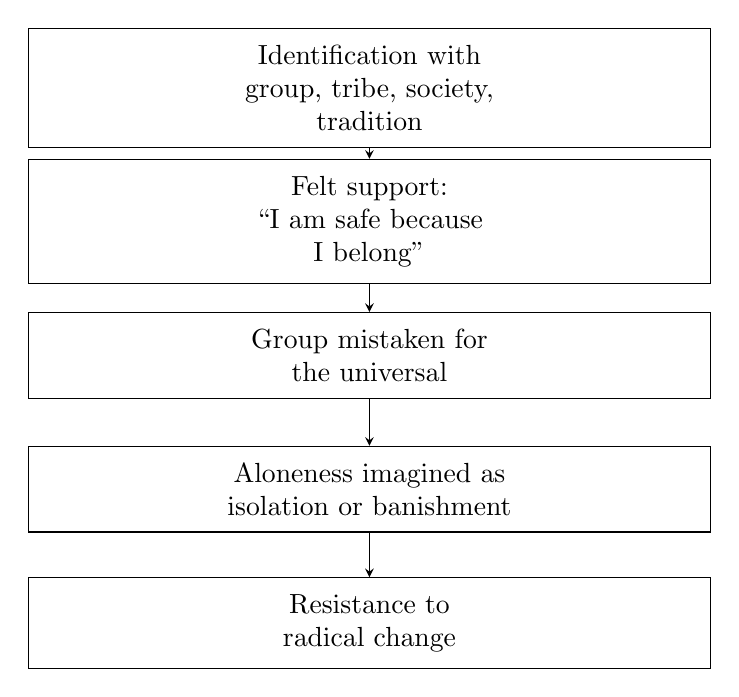
\begin{tikzpicture}[>=stealth, every node/.style={draw, align=center, text width=.68\linewidth, inner sep=6pt}, node distance=1.6cm]
\node (a) at (0,0) {Identification with\\group, tribe, society,\\tradition};
\node (b) at (0,-1.7) {Felt support:\\``I am safe because\\I belong''};
\node (c) at (0,-3.4) {Group mistaken for\\the universal};
\node (d) at (0,-5.1) {Aloneness imagined as\\isolation or banishment};
\node (e) at (0,-6.8) {Resistance to\\radical change};
\draw[->] (a) -- (b);
\draw[->] (b) -- (c);
\draw[->] (c) -- (d);
\draw[->] (d) -- (e);
\end{tikzpicture}

Transcript-derived schematic of the first obstacle to change. It is not a board diagram from the video.
\end{figure}

\section{The Group as False Universal}

The lecture then makes the decisive move. It is not enough to say that people like company or fear loneliness. The group has become the self. In the dialogue this is put starkly: the group is me; I am the group.

A compact way to preserve this step is:
\begin{equation}
\text{group} \neq \text{universal},
\qquad
\text{but the group is felt as universal support}.
\end{equation}

The point is not sociological classification. It is the felt logic of dependence. The child may take the tribe or town as the whole world. The adult may know abstractly that the group is not the whole, while feeling that without the group there is no orientation. To be banished from it is not merely to lose company. It can feel like losing one's being.

The dialogue even revises a familiar philosophical gesture. Instead of ``I think, therefore I am,'' the group-bound mind says, in effect:
\begin{equation}
\text{I am in the group} \longrightarrow \text{I am}.
\end{equation}

This is why banishment has such force. The person outside the group does not merely lack approval; he does not know where he is. The map by which he has lived no longer locates him.

\subsection{Question \& Answer}

\paragraph{Question.}
If one is alone, is one cut off from the universal?

\paragraph{Answer.}
The lecture answers in the opposite direction. What is cut off is the person identified with a false universal. The group has been treated as though it were the whole, as though it were the support of being. Genuine aloneness is not separation from the universal; it begins when the false identification with the group is seen and dropped.

\section{Aloneness Is Not Isolation}

The lecture now gives aloneness a sharper meaning. Aloneness is not the private feeling of being apart. It is not loneliness, exile, or psychological abandonment. It means stepping out of the stream: the stream of confusion, disorder, sorrow, despair, hope, travail, and the known. To go deeper, it means not carrying the burden of tradition.

The core distinction is therefore:
\begin{equation}
\text{aloneness} \neq \text{isolation}.
\end{equation}

Isolation belongs to the image of being unsupported. Aloneness belongs to freedom from the structure that has made support necessary. The dialogue connects tradition and knowledge to the group because knowledge, in the psychological sense being examined here, is collective accumulation. One carries the past, the inherited answer, the accepted pattern.

So the movement is not:
\begin{equation}
\text{group} \longrightarrow \text{private isolation}.
\end{equation}
It is rather:
\begin{equation}
\text{group/tradition/known}
\longrightarrow
\text{freedom from the stream}.
\end{equation}

This is why the lecture can say that aloneness implies total freedom. That statement should not be made at the beginning of the chapter as a slogan. It has to be earned through the preceding distinction: the mind is not escaping relationship; it is no longer depending on the false relationship of identification.

\section{Chaos, Cosmos, and the Danger of Consolation}

At this point the dialogue risks becoming too easy. If aloneness is freedom, and freedom is connected with the universal, why not say simply: you are the universe? Krishnamurti rejects that as dangerous when the person saying it is in confusion.

The correction is exact:
\begin{equation}
\text{cosmos} = \text{order},
\qquad
\text{chaos} = \text{disorder and confusion}.
\end{equation}

The Greek note appears only to sharpen the contrast. Cosmos means order; chaos is its opposite. Therefore one cannot claim universal order while living in disorder, anxiety, jealousy, misery, and fragmentation. To say, ``inside there is perfect order,'' while disorder is actual, is a projection by thought. It gives hope, but it does not give actuality.

The lecture's discipline is to begin with what is so:
\begin{equation}
\text{actual starting point} = \text{fact of chaos},
\end{equation}
not:
\begin{equation}
\text{actual starting point} = \text{projected cosmos}.
\end{equation}

\subsection{Question \& Answer}

\paragraph{Question.}
Can one say, ``I am the universe,'' while living in confusion?

\paragraph{Answer.}
No. The lecture treats that as one of thought's consoling tricks. If one is confused, the fact is confusion. A projected cosmos is still part of thought's movement within chaos. Order cannot be borrowed as an idea. One must begin with the fact of what one is.

From here the phrase ``alone'' is clarified again. When there is order, there is no fragmentation. The word ``alone'' is heard as ``all one,'' not as isolated existence. If there is cosmos, there are not separate psychological centers preserving division under a spiritual name. There is order, and order is alone.

\section{Thought, Reality, and the Corporation Called Me}

Having traced the fear of change through group, false security, and chaos, the dialogue turns inward. Why do human beings not change? Another answer appears: we are conditioned to accept things as they are. Even the phrase ``this is all that can be'' closes the inquiry. The word ``all'' gives completeness to a condition that may only be habit. It turns an idea into apparent reality.

Religions may project another world. Political systems may project a future world. In both cases, thought invents a place to go, and that place is made from the old movement. It is a subtle way of not being alone.

The inquiry then asks the question directly: why do you not change? The answer is not available because the question has not been asked radically. This brings the lecture to thought itself. Society, religion, culture, and the search for outside agency are all based on thought. Thought says, ``I cannot do this,'' and therefore seeks the environment, the leader, God, or history to change it. Yet the same old me remains.

The central relation is:
\begin{equation}
\text{thought} \longrightarrow \text{me},
\qquad
\text{not}
\qquad
\text{me} \longrightarrow \text{thought}.
\end{equation}

The corporation analogy gives this relation a vivid form. A corporation is treated as though it were independently real. It makes money, loses money, pays taxes, owns buildings, and survives the loss of particular buildings. Yet its reality depends on a whole movement of thought, law, agreement, and recognition. In the same way, thought creates the ``me'' and then treats the ``me'' as an independent source.

The mistaken reversal can be written:
\begin{equation}
\text{thought creates me}
\quad \text{but then says} \quad
\text{me creates thought}.
\end{equation}

This is the structure of ``thinking incorporated.'' Credit for thought is assigned to the corporation called me. But the me is not separate from thought. It is the structure of thought.

\section{Thought as Movement, Time, and the End of Me}

The lecture now returns to the question that had been left unfinished: does thought see itself in movement? The wording matters. It is not, ``I am aware of thought as movement,'' because the ``I'' has itself been created by thought. The question is whether thought is aware of itself as movement.

The late conceptual spine is:
\begin{align}
\text{thought} &= \text{movement}, \\
\text{movement} &= \text{time}, \\
\text{me} &= \text{time put together by thought}.
\end{align}

Movement means from here to there. Physically, it is from here to London or New York. Psychologically, it is ``I am this; I must be that.'' This is time as psychological becoming. The me is not an entity standing outside this movement. The me is the continuity of the movement.

\subsection{Question \& Answer}

\paragraph{Question.}
Does thought see itself as movement, or does an ``I'' see thought?

\paragraph{Answer.}
The lecture rejects the second formulation. If the ``I'' sees thought, the structure has already been divided into observer and observed. But the ``I'' is itself made by thought. The actual question is whether thought realizes its own movement without creating a separate observer to claim the realization.

\paragraph{A worked schematic.}
The dialogue describes a feedback loop. A person says, ``I have a problem; I am suffering.'' The thought includes an implicit ``I'' who is real, and because the ``I'' is felt as real, the suffering is felt as real in a way that demands more thought. The next thought then says that the problem must be thought about further. This sustains the very structure that suffers.

As a schematic reconstruction:
\begin{align}
T_0 &: \quad \text{``I am suffering''}, \\
T_1 &: \quad \text{``Since I am real, this suffering is real''}, \\
T_2 &: \quad \text{``Since it is real, I must think more''}, \\
T_3 &: \quad \text{further thought sustaining the same } I.
\end{align}

Or more compactly:
\begin{equation}
\text{thought}
\longrightarrow
\text{image of me}
\longrightarrow
\text{sense of reality}
\longrightarrow
\text{further thought}.
\end{equation}

This is not a mechanical law. It is a note-form version of the dialogue's point: thought feeds on the reality it has itself projected. If the movement stops, the sense of me as a continuing psychological entity has no independent basis.

The lecture then draws a distinction that must be preserved. When the movement of psychological thought ends, this does not mean the brain can no longer use technical thought. Technical thought can function in order. What ends is the movement that creates the me, division, and fear.

\begin{equation}
\text{thought as movement}
\longrightarrow
\text{fragmentary action},
\end{equation}
while
\begin{equation}
\text{ending of thought-as-movement}
\longrightarrow
\text{total action}.
\end{equation}

The phrase ``total action'' is not defined as a technique. It is the lecture's contrast to action born from division.

\section{Fact, Fear, and Remaining With What Is}

The closing movement turns the whole inquiry toward fear. If thought as movement ends, the me ends. That is felt as death, not merely biological death, but the ending now of everything thought has put together: knowledge, possessions, relations as images, continuity, and the known self.

The lecture then asks how this is received. Panic appears. A fear of death appears. But Krishnamurti presses the distinction between the actuality of the fact and the word or image that awakens fear. The key relation is:

\begin{equation}
\text{fact} \longrightarrow \text{no fear}.
\end{equation}

Fear begins when thought makes an abstraction, a picture of ending:
\begin{equation}
\text{fact}
\longrightarrow
\text{abstraction/image}
\longrightarrow
\text{fear}.
\end{equation}

This is the chapter's sharpest equation. It must not be softened into general advice about courage. The lecture is saying something more precise: when the actuality of the fact is present, there is no fear. Fear comes when thought moves away from the fact and makes an image of it.

\subsection{Question \& Answer}

\paragraph{Question.}
What happens when the fact is actually seen?

\paragraph{Answer.}
There is no fear. Fear is not in the fact itself. Fear is in the idea brought about by abstraction, in the picture of ending. As soon as thought comes in, one is no longer with the fact. One is with imagination, fantasy, or a felt reality produced by thought.

The dialogue briefly states this in its strongest form: all fear is thought, and all thought is fear or sorrow. The chapter must hear that with the immediate qualification already present in the discussion. Technical thought may still operate in order. The thought being examined is psychological movement: image, continuity, becoming, and the me.

To remain with the fact is not to explain it away, not to say it should or should not be, not to move into self-pity or method. The example given is sorrow: can one remain totally with sorrow without moving away? If so, the lecture says, there is an extraordinary energy.

\section{Summary}

The lecture begins with a practical unfinished question: why do human beings not change? It first shows that change threatens both real security and the psychological security of belonging. The group is then exposed as a false universal: it supports the feeling of being, but it is not the universal; it belongs to fragmentation.

From there, aloneness is distinguished from isolation. Aloneness means freedom from the stream of the known, tradition, and collective psychological dependence. This leads to the severe correction that cosmos means order, and one must not project order while living in chaos.

The final movement discovers the deeper source of the problem in thought. Thought creates the me and treats it as independently real. Thought is movement; movement is time; the me is time put together by thought. The ending of that movement is feared as death. Yet when the fact is actually present, there is no fear. Fear begins when thought makes an image of the fact and moves away from it.